%--------------------------%
\section{January 2023} %---%
%--------------------------%

%%%%%%%%%%%%%%%%%%%%%%%%%%%%%%%%%%%%%
\subsection*{Classical Mechanics} %%%
%%%%%%%%%%%%%%%%%%%%%%%%%%%%%%%%%%%%%
\addcontentsline{toc}{subsection}{Classical Mechanics}

\prob{1.1}{

A spherical bathyscaphe of mass $M$ and radius $R$ is moving underwater with the velocity $v_0$ parallel to the surface.
At $t = 0$ the engine stops and the bathyscaphe pops up.
Assuming that at $t = 0$ the bathyscaphe was at the distance $h$ from the surface, as shown in the figure below, obtain equations for:

\begin{parts}
    \item The time $T$ for the bathyscaphe to emerge at the surface after the engine stops.

    \item The lateral distance $L$ the bathyscaphe travels before it pops up.
\end{parts}

Assume that: (1) the water has the mass density $\rho$ and $M < 4 \pi R^2 \rho / 3$, (2) The drag force acting on the bathyscaphe $\vb*{F} = - \gamma \vb*{v}$ is proportional to its velocity $\vb*{v}$, where $\gamma$ is a positive constant.

Solve the equations for $T$ and $L$ in the limit of $T \gg M/\gamma$.

\begin{center}
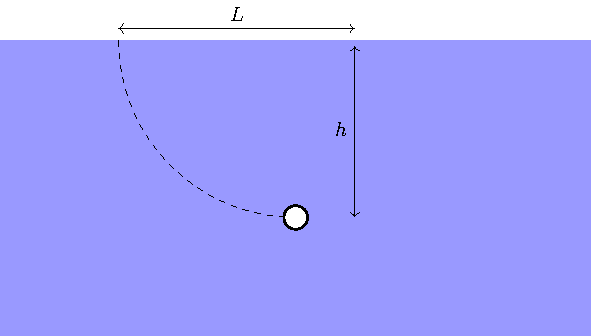
\includegraphics{January2023/1-1.pdf}
\end{center}

}

\sol{}


\prob{1.2}{

A thin-shelled sphere of radius $\rho$ and mass $m$ is constrained to roll without slipping on the lower half of the inner surface of a hollow, stationary cylinder of radius $R$.

Take $\theta$ to be the generalized coordinate and use $I = \frac{2}{3} m \rho^2$ to find the Lagrange equation of motion that describes the motion of the shell.

\begin{center}
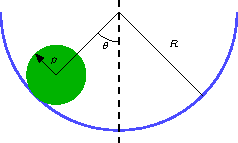
\includegraphics{January2023/1-2.pdf}
\end{center}

}

\sol{}


\prob{1.3}{

An ideal (flexible, uniform, frictionless, etc.) rope of length $l$ and mass $M$ starts sliding off an ideal frictionless table as shown in the figure (the rope is initially at rest, the gravitational accleration is $g$, the size of the piece of the rope initially hanging off the table is $y_0$).

\begin{center}
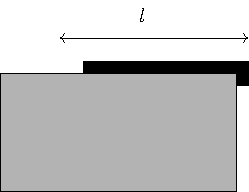
\includegraphics{January2023/1-3.pdf}
\end{center}

\begin{parts}
    \item Introduce some generalized coordinate and write down the Lagrangian of the system.

    \item Derive the Euler-Lagrange equations of motion.

    \item Calculate the time $\tau$ for the rope to slide half-way off the table.
\end{parts}

}

\sol{}


\prob{1.4}{

A smooth wire is bent into the shape of a spiral helix with a decreasing pitch.
In cylindrical polar coordinates $(\rho,\phi,z)$ it is specified by equations $\rho = R$ and $z = \lambda \sqrt{\phi}$, where $R$ and $\lambda$ are positive constants.
The $z$ axis is vertically up (and gravity vertically down).

\begin{parts}
    \item Using $z$ as a generalized coordinate, write down the Lagrangian for a bead of mass $m$ threaded on the wire.

    \item Find the Lagrange equation and calculate the bead's vertical acceleration $\ddot{z}$ as a function of $z$ and $\dot{z}$.

    \item Find aceleration $\ddot{z}$ in two limits: (i) when $R \rightarrow 0$ but $\lambda$ is fixed, and (ii) when $\lambda \rightarrow \infty$ but $R$ is fixed.
    Discuss if the results for $\ddot{z}$ in these limits make sense.
\end{parts}

}

\sol{}


\prob{2.1}{

You are told that, at the known positions $x_1$ and $x_2$, an oscillating mass $m$ has speeds $v_1$ and $v_2$.
What are the amplitude and the angular frequency of the oscillations?

}

\sol{}

%%%%%%%%%%%%%%%%%%%%%%%%%%%%%%%%%%%%%%%%%%
\subsection*{Electricity \& Magnetism} %%%
%%%%%%%%%%%%%%%%%%%%%%%%%%%%%%%%%%%%%%%%%%
\addcontentsline{toc}{subsection}{Electricity \& Magnetism}

\prob{2.2}{

An electron with mass $m_e$ and momentum $p_e$ hits a positron at rest.
They annihilate, producing a pair of photons.
If one of the photons emerge at angle $\theta$ to the incident electron direction, what is the second photon's angle?

}

\sol{}


\prob{2.3}{

A toroid is a ``donut'' shaped coil, and the figure below shows an overhead cross sectional view of one.
They are used in nuclear fusion reactors called tokamaks.
Use Ampere's law to derive the equation for the magnitude of the magnetic field in a toroid ($N$ turns) of inner radius $a$ and outer radius $b$ at a distance $r$ midway between $a$ and $b$.

Express your result in terms of $a$, $b$, current $I$, $N$ and any constants.

\begin{center}
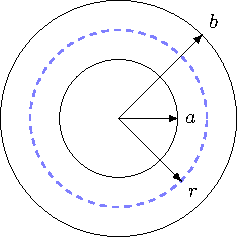
\includegraphics{January2023/2-3.pdf}
\end{center}

}

\sol{}


\prob{2.4}{

A small neutral metallic conducting sphere with radius $a$ is separated by a transverse distance $R \gg a$ from an infinitely long wire of negligible thicknes and charge per unit length $\lambda$.

\begin{center}
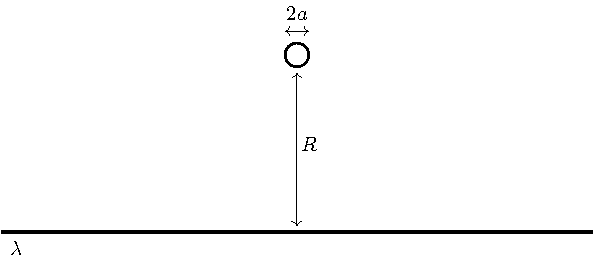
\includegraphics{January2023/2-4.pdf}
\end{center}

Calculate the force between the metallic sphere and the wire.

\textbf{Hint}: Recall the induced electric dipole moment of a conducting sphere in a uniform electric field $\vb*{E}$ is $\vb*{p} = 4 \pi a^3 \vb*{E}$.

}

\sol{}


\prob{3.1}{

The $\psi'$ particle, which is a bound state $\bar{c}c$ of charmed quarks, has mass approximately equal to $3.7~{\rm GeV}/c^2$.

What is the minimal (``threshold'') energy of photons necessary to produce $\psi'$ particles in the reaction $\gamma p \rightarrow p \psi'$ from the Hall D photon source at JLab accelerator?

}

\sol{}


\prob{3.2}{

A cylinder of radius $\rho = a$ carries an azimuthal surface current $\vb*{K} = f(z) \hat{\phi}$ where $f(z)$ is an arbitrary function, in cylindrical coordinate $(\rho,\phi,z)$.

Find expressions for $\vb*{B}(0)$, the magnetic field at the origin, and $\vb*{m}$, the magnetic moment of the system, as integrals involving $f(z)$.

}

\sol{}


\prob{3.3}{

Consider two semi-infinite dielectric media with permittivities $\epsilon_1$ at $x < 0$ and $\epsilon_2$ at $x > 0$.
Let a charge $q$ be in a medium 1 at $x_0 = -L$, where $L$ is a distance between the charge and the planar interface $x = 0$ between the media.
Calculate:

\begin{parts}
    \item The electric potential $\varphi(x,y,z)$ in the entire space.

    \item The force $F$ acting on the charge.
\end{parts}

\begin{center}
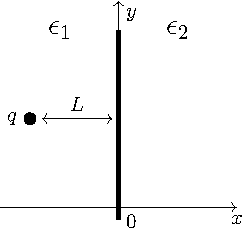
\includegraphics{January2023/3-3.pdf}
\end{center}

}

\sol{}

%%%%%%%%%%%%%%%%%%%%%%%%%%%%%%%%%%%
\subsection*{Quantum Mechanics} %%%
%%%%%%%%%%%%%%%%%%%%%%%%%%%%%%%%%%%
\addcontentsline{toc}{subsection}{Quantum Mechanics}

\prob{3.4}{

A particle with spin $S = 1$ is in a state described by the following bra-vector in the $\hat{S}_z$ basis:
\begin{align*}
    \bra{\psi} = \frac{1}{\sqrt{14}} (-i,2,3)
\end{align*}

\begin{parts}
    \item Calculate the probabilities that a measurements of $S_z$ wll give 1, 0, and -1.

    \item Calculate the expectation values of $\expval{S_z}$, $\expval{S_y}$, and $\expval{S_z}$.
\end{parts}

\textbf{Hint}: The spin-1 matrices are
\begin{align*}
    \hat{S}_x = \frac{\hbar}{\sqrt{2}}\begin{pmatrix}
        0 & 1 & 0 \\
        1 & 0 & 1 \\
        0 & 1 & 0
    \end{pmatrix}
    ,\quad
    \hat{S}_y = \frac{\hbar}{\sqrt{2}}\begin{pmatrix}
    0 & -i & 0 \\
    i & 0 & -i \\
    0 & i & 0
    \end{pmatrix}
    , \quad
    \hat{S}_z = \hbar
    \begin{pmatrix}
        1 & 0 & 0 \\
        0 & 0 & 0 \\
        0 & 0 & -1
    \end{pmatrix}
\end{align*}

}

\sol{}


\prob{4.1}{

Consider a particle of mass $m$ subject to a $\delta$-function potential given by
\begin{align*}
    V(x) = -\frac{\hbar^2}{2m} v_0 \delta(x)
.\end{align*}
Suppose the particle is initially in the bound state.
Suddenly, the potential $V(x)$ is changed to $\overline{V}(x)$ by increasing the strength $v_0 \rightarrow \overline{v}_0$.
Assume that this sudden change does not affect the state of the particle.
Compute the probability that the particle remains in the ground state corresponding to the potential $\overline{V}(x)$.
Why is this probability less than one?

Evaluate the expectation value of the Hamiltonian with the potential $\overline{V}(x)$ and obtain the energy required to change $V(x) \rightarrow \overline{V}(x)$.

}

\sol{}


\prob{4.2}{

Consider a hydrogen atom exposed to a uniform electric field $\mathcal{E} \hat{z}$ (ignore spin degrees of freedom).
Calculate the corrections to the ground-state energy level up to second order in perturbation theory.
You may neglect the contribution from the continuum states in the second-order calculation.

Exploiting selection rules based on parity and $L_z$, you will realize that you only need the following ground- and excited-state wave functions to carry out this calculation,
\begin{align*}
    \phi_{100}(r) = R_{10}(r) \underbrace{\frac{1}{\sqrt{4 \pi}}}_{Y_{00}}, \quad \phi_{n10}(r) = R_{n1}(r) \underbrace{\sqrt{\frac{3}{4 \pi}} \cos{\theta}}_{Y_{10}}
\end{align*}
Express the result in terms of the overlap integral
\begin{align*}
    \gamma_n = \int_{0}^{\infty} \dd{r} \, r^3 R_{n1}(r) R_{10}(r)
.\end{align*}
Note that you do not need to evaluate this integral!

}

\sol{}


\prob{4.3}{

Consider a system with a three-dimensional state space.
The Hamiltonian $\hat{H}$ has a non-degenerate eigenvalue $E_1$ with (normalized) eigenstate $\ket{\phi_1}$ and a degenerate eigenvalue $E_2$ with (orthonormal) eigenstates $\ket{\phi_2}$ and $\ket{\phi_3}$.
Suppose at time $t = 0$, the system is in the normalized state $\ket{\psi(0)}$ given by
\begin{align*}
    \ket{\psi(0)} = \frac{1}{\sqrt{2}} \ket{\phi_1} + \frac{1}{2} ( \ket{\phi_2} + \ket{\phi_3} )
.\end{align*}

\begin{parts}
    \item At $t = 0$ the energy of the system is measured.
    What values can be found and with what probabilities?

    \item Suppose at $t = 0$, instead of $\hat{H}$, the observable $\hat{A}$, which in the basis $\ket{\phi_1}$, $\ket{\phi_2}$, and $\ket{\phi_3}$ is represented by the following matrix
    \begin{align*}
        A = a \begin{pmatrix}
            1 & 0 & 0 \\
            0 & 0 & 1 \\
            0 & 1 & 0
        \end{pmatrix}
    ,\end{align*}
    where $a > 0$ is real, is measured with the system in state $\ket{\psi(0)}$.
    What results can be found and with what probabilities?
    Do $\hat{H}$ and $\hat{A}$ commute?

    \item What is the mean value $\bra{\psi(t)} \hat{A} \ket{\psi(t)}$?
\end{parts}

}

\sol{}


\prob{4.4}{

Consider a system with a two-dimensional state space.
In this space, the states $\ket{1}$ and $\ket{2}$ form an orthonormal basis.
The Hamiltonian describing the system in this basis has the form
\begin{align*}
    \hat{H} = H_{11} \ket{1}\bra{1} + H_{22} \ket{2}\bra{2} + H_{12} ( \ket{1}\bra{2} + \ket{2}\bra{1} )
,\end{align*}
where $H_{11}$, $H_{22}$, and $H_{12}$ are real parameters with dimension of energy.

\begin{parts}
    \item Assume $H_{12} = 0$.
    Write down the eigenvalues and eigenvectors of $\hat{H}$ in the basis $\ket{1}$, $\ket{2}$.

    \item Now, assume $H_{12} \ne 0$.
    Obtain the eigenvalues and corresponding eigenvectors of $\hat{H}$.
    Make sure that they reduce to the eigenvalues and eigenvectors of part (a) above in the limit $H_{12} \rightarrow 0$.
    It is convenient to introduce the parameter
    \begin{align*}
        \lambda = \frac{2 H_{12}}{H_{11} - H_{22}} \quad {\rm with}~ H_{11} \ne H_{22}
    ,\end{align*}
    and express results in terms of $\lambda$.
\end{parts}

}

\sol{}